\documentclass[linenumbers]{aastex63}
\usepackage{graphicx} % Required for inserting images
\usepackage{natbib}


\begin{document}

\title{ASTR 400B Research Assignment 2 \\
MW/M31 Galaxy Major Merger Remnant: Stellar disk particle kinematics}

\author[0000-0002-4901-7693]{Charlie Goldberg}

\affiliation{Steward Observatory \\
937 N. Cherry Ave \\
Tucson, AZ 85719, USA}

\section{Introduction}

The purpose of this project is to understand the remains of mergers between two large spiral galaxies. Specifically, this project will analyze the remnant of the Milky Way-Andromeda collision to determine if its kinematics resemble those of observed elliptical galaxies.\\

This topic is important because the formation mechanism of elliptical galaxies is not fully understood, yet they make up over 10\% of all known galaxies (\cite{1996MNRAS.278.1025L}). By simulating galaxy mergers and studying their products, the formation of elliptical galaxies can be better understood.\\

It is currently known that elliptical galaxies often result from mergers between spiral galaxies (\cite{2006ApJ...650..791C}). In addition, the largest elliptical galaxies are thought to be the result of several mergers (\cite{2006ApJ...650..791C}).\\

While the general formation mechanism of elliptical galaxies is understood, it is unclear why ellipticals have little rotation (\cite{1998A&AS..133..325G}) while their progenitors do. In addition, it is not understood why smaller elliptical galaxies rotate more than their larger counterparts (\cite{2011MNRAS.414..888E}). Finally, it is unknown why many elliptical galaxies do not appear to be dark matter dominated, despite their progenitors being heavily dominated by dark matter (\cite{2003Sci...301.1696R}).

\begin{figure}
    \centering
    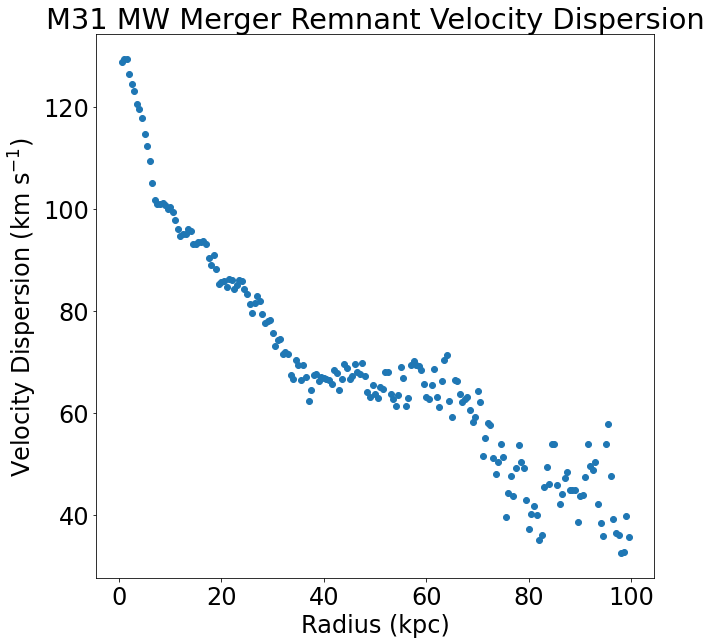
\includegraphics[width=0.5\textwidth]{dispersion.jpg}
    \caption{Image of NGC 3379 showing the relative velocities of planetary nebulae within the galaxy. The motion of the nebulae toward and away from the observer appears random, indicating the galaxy has little or no rotation. Figure from \cite{2003Sci...301.1696R}.}
    \label{dispersion}
\end{figure}

\section{Proposal}

\subsection{}
I will address two questions: Does the merger remnant rotate, and does the remnant have a velocity dispersion typical of large or small ellipticals? Answering these questions will help us understand if large galaxy mergers such as the one between the Milky Way and Andromeda are capable of producing elliptical galaxies similar to the ones we observe.

\subsection{}

To determine if the merger remnant rotates, I will have to analyze the particles from both the Milky Way and Andromeda and find the center of mass of the new galaxy. I will define this as the origin for a spherical coordinate system and find the $\hat{\phi}$ and $\hat{\theta}$ components of velocity for each object. I will then create histograms showing the component velocities of each object. I will not know the orientation of the galaxy with respect to the coordinate system, however, if the galaxy is rotating the majority of particles will have the same sign of either $\hat{\phi}$ or $\hat{\theta}$ velocity. If the galaxy is not rotating and the particles all orbit in random directions, there will be no preference for a positive or negative velocity.\\

To determine the velocity dispersion of the merger remnant as a function of radius, I will once again combine the particle data from the Milky Way and Andromeda and find the new center of mass. Then at increasing distances from the center of mass I will find the standard deviation of the magnitude of velocity for all particles at the specified radius.\\

\begin{figure}
    \centering
    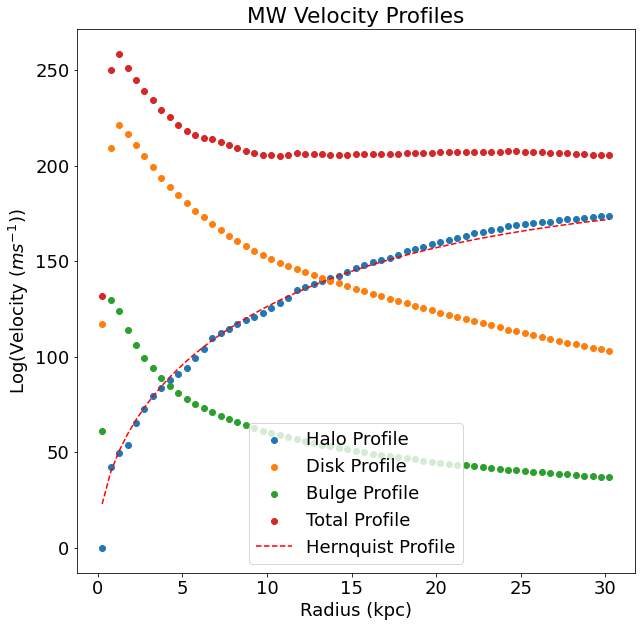
\includegraphics[width=0.6\textwidth]{mw_velo.png}
    \caption{This image shows the velocity of particles as a function of radius for the Milky Way. For this project I will create a similar plot, but for the velocity dispersion of the merger remnant.}
    \label{velocity}
\end{figure}

\subsection{}

Because the Milky Way and Andromeda are inclined to each other, and because the merger in the simulation is collisionless, I predict that most of the stars will orbit in random directions, resulting in little or no net rotation. This is typically observed in large ellipticals similar to the merger remnant.\\

Finally, I predict that that the velocity dispersion will be greatest near the center of the remnant and decrease at larger radii because there are many more particles near the core, allowing for greater variations in velocity. In addition, the particle velocities are much higher near the core, so a small percentage deviation from the mean velocity results in a larger change in velocity. A higher dispersion near the core is also observed in many ellipticals.

\bibliography{references.bib}{}
\bibliographystyle{aasjournal}

\end{document}
